\documentclass[a4paper]{book}

\usepackage{latexsym, amssymb}
\usepackage{graphicx}
%\usepackage{longtable}
\usepackage{supertabular}
%\usepackage{tabularx}
%\usepackage{tabulary}
%\usepackage{rail}
%\railoptions{-t -h}
\usepackage{xspace}
\usepackage[rounded]{syntax}
\usepackage{hyperref}
\usepackage{listings}
\usepackage[usenames]{color} 

\relax

\begin{document}

\definecolor{yobg}{rgb}{0.9,0.9,1}
\definecolor{yotxt}{rgb}{0.01,0.01,0.52}
\definecolor{mylstcmt}{rgb}{0.01,0.52,0.01} % a dark green.
%%\newcommand{\farg}[1]{\textrm{\textit{#1}}}

% parameters for listings
\lstset{
	tabsize=4,
	showspaces=false,
	showstringspaces=false,
    language=C++, 
    basicstyle=\ttfamily\color{yotxt},
    numbers=none,
    stepnumber=2,
  commentstyle=\slshape\color{mylstcmt},
    %%frame=single,
    backgroundcolor=\color{yobg},
    captionpos=b
}

\title{\faust Quick Reference}
\author{Yann Orlarey\\\textsc{Grame} -- Centre National de Cr\'eation Musicale}
\date{December 2009}


% \railalias{recur}{$\sim$}
% \railalias{lbrace}{\{}
% \railalias{rbrace}{\}}
% \railalias{dollar}{\$}
% \railalias{mod}{\%}
% \railalias{arobase}{@}
% \railalias{ampersand}{\&}
% \railalias{hat}{$\land$}
% \railalias{kot}{'}
% \railalias{pipe}{$|$}
% \railalias{fdelay}{}
% \railalias{backslash}{\char"5C}
% \railterm{recur,lbrace,rbrace,dollar,mod,kot,arobase,ampersand,backslash,fdelay, pipe, hat}

\newcommand{\farg}[1]{\textrm{\textit{#1}}}
\newcommand{\ldbrack}{[\![ \,}
\newcommand{\rdbrack}{\, ]\!] }
\newcommand{\rdbrackC}{\rdbrack_{\mathrm{C}}\,}
\newcommand{\dbrack}[1]{\ldbrack #1 \rdbrack}
\newcommand{\semantic}[1]{\ldbrack #1 \rdbrack}
\newcommand{\dbrackC}[1]{\ldbrack #1 \rdbrackC}

\newcommand{\faust}{\textsc{Faust}\xspace}
\newcommand{\latex}{\LaTeX\xspace}

\setlength{\parindent}{0pt}
\setlength{\parskip}{1ex plus 0.5ex minus 0.2ex}

\maketitle


\chapter{Introduction}

\faust (\textit{Functional Audio Stream}) is a functional programming language specifically designed for real-time signal processing and synthesis.  \faust targets high-performance signal processing applications and audio plug-ins for a variety of platforms and standards. 

\section{Design Principles}

Various principles have guided the design of \faust :

\begin{itemize}

\item \faust is a \textit{specification language}. It aims at providing an adequate notation to describe \textit{signal processors} from a mathematical point of view. It is, as much as possible, free from implementation details. 

\item \faust programs are fully compiled, not interpreted. The compiler translates \faust programs into equivalent C++ programs taking care of generating the most efficient code. The result can generally compete with, and sometimes even outperform, C++ code written by seasoned programmers. 

\item The generated code works at the sample level. It is therefore suited to implement low-level DSP functions like recursive filters. Moreover the code can be easily embedded. It is self-contained and doesn't depend of any DSP library or runtime system. It has a very deterministic behavior and a constant memory footprint. 

\item The semantic of \faust is simple and well defined. This is not just of academic interest. It allows the \faust compiler to be \emph{semantically driven}. Instead of compiling a program literally, it compiles the mathematical function it denotes. This feature is useful for example to promote components reuse while preserving optimal performance.  

\item \faust is a textual language but nevertheless block-diagram oriented. It actually combines two approaches: \textit{functional programming} and \textit{algebraic block-diagrams}. The key idea is to view block-diagram construction as function composition. For that purpose, \faust relies on a \emph{block-diagram algebra} of five composition operations (\lstinline': , ~ <: :>').

\item Thanks to the notion of \textit{architecture}, \faust programs can be easily deployed on a large variety of audio platforms and plugin formats without any change to the \faust code.

\end{itemize}

\section{Signal Processor Semantic}
A \faust program describes a \emph{signal processor}. The role of a \textit{signal processor} is to transforms a group  of (possibly empty) \emph{input signals} in order to produce a group of (possibly empty) \emph{output signals}. 

More precisely :

\begin{itemize}

\item A \emph{signal} $s$ is a discrete function of time $s:\mathbb{N}\rightarrow\mathbb{R}$. 
The value of signal $s$ at time $t$ is written $s(t)$. 
The set $\mathbb{S}=\mathbb{N}\rightarrow\mathbb{R}$ is the set of all possible  signals.

\item A group of $n$ signals (a \emph{n}-tuple of signals) is written
$(s_{1},\ldots,s_{n})\in \mathbb{S}^{n}$.
The \emph{empty tuple}, single element of $\mathbb{S}^{0}$ is notated  $()$.

\item A \emph{signal processors} $p$, is a function from
\emph{n}-tuples of signals to \emph{m}-tuples of signals
$p:\mathbb{S}^{n}\rightarrow\mathbb{S}^{m}$. The set $\mathbb{P}=\bigcup_{n,m}\mathbb{S}^{n}\rightarrow\mathbb{S}^{m}$ is the
set of all possible signal processors.

\end{itemize}

As an example, let's express the semantic of the \faust primitive \lstinline'+'. Like any \faust expression, it is a signal processor. Its signature is $\mathbb{S}^{2}\rightarrow\mathbb{S}$. It takes two input signals $X_0$ and $X_1$ and produce an output signal $Y$ such that $Y(t) = X_0(t)+X_1(t)$. 

Numbers are signal processors too. For example the number $3$ has signature  $\mathbb{S}^{0}\rightarrow\mathbb{S}$.  It takes no input signals and produce an output signal $Y$ such that $Y(t) = 3$. 

\chapter{Compiling and installing \faust}

The \faust source distribution \lstinline'faust-0.9.10.tar.gz' can be downloaded from sourceforge (\url{http://sourceforge.net/projects/faudiostream/}).

\section{Organization of the distribution}
The first thing is to decompress the downloaded archive. 
\begin{lstlisting}
	tar xzf faust-0.9.10.tar.gz
\end{lstlisting}

The resulting  \lstinline'faust-0.9.10/' folder should contain the following elements:

\begin{tabular}{ll}
	\lstinline'architecture/' 		&\faust libraries and architecture files\\
	\lstinline'benchmark'			&tools to measure the efficiency of the generated code\\
	\lstinline'compiler/'			&sources of the \faust compiler\\
	\lstinline'examples/'			&examples of \faust programs\\
	\lstinline'syntax-highlighting/'&	support for syntax highlighting for several editors\\
	\lstinline'documentation/' 		&\faust's documentation, including this manual\\
	\lstinline'tools/'				&tools to produce audio applications and plugins\\
	\lstinline'COPYING'				&license information\\
	\lstinline'Makefile'			&Makefile used to build and install \faust\\
	\lstinline'README'				&instructions on how to build and install \faust
\end{tabular}

\section{Compilation}
\faust has no dependencies outside standard libraries. Therefore the compilation should be straightforward. There is no configuration phase, to compile the \faust compiler simply do :
\begin{lstlisting}
	cd faust-0.9.10/
	make
\end{lstlisting}

If the compilation was successful you can test the compiler before installing it:
\begin{lstlisting}
	[cd faust-0.9.10/]
	./compiler/faust -v
\end{lstlisting}
It should output:
\begin{lstlisting}
	FAUST, DSP to C++ compiler, Version 0.9.10
	Copyright (C) 2002-2010, GRAME - Centre... 
\end{lstlisting}

Then you can also try to compile one of the examples :
\begin{lstlisting}
	[cd faust-0.9.10/]
	./compiler/faust examples/noise.dsp
\end{lstlisting}
It should produce some C++ code on the standard output

\section{Installation}
You can install \faust with:
\begin{lstlisting}
	[cd faust-0.9.10/]
	sudo make install
\end{lstlisting}
or
\begin{lstlisting}
	[cd faust-0.9.10/]
	su
	make install
\end{lstlisting}
depending on your system.


\section{Compilation of the examples}
Once \faust correctly installed, you can have a look at the provided examples in the \lstinline'examples/' folder. This folder contains a  \lstinline'Makefile' with all the required instructions to build these examples for various \textit{architectures}\footnote{an architecture file provides the code to connect a signal processor to the outside world (audio communications and user interface)}, either standalone audio applications or plugins.

The command \lstinline'make help' will list the available targets. Before using a specific target, make sure you have the appropriate development tools, libraries and headers installed. For example to compile the examples as ALSA applications with a GTK user interface do a \lstinline'make alsagtk'. This will create a \lstinline'alsagtkdir/' subfolder with all the binaries. 


\chapter{\faust syntax}

This section describes the syntax of \faust. Figure \ref{fig:syntax} gives an overview of the various concepts and where they are defined in this section. 

\begin{figure}[ht!]
\centering
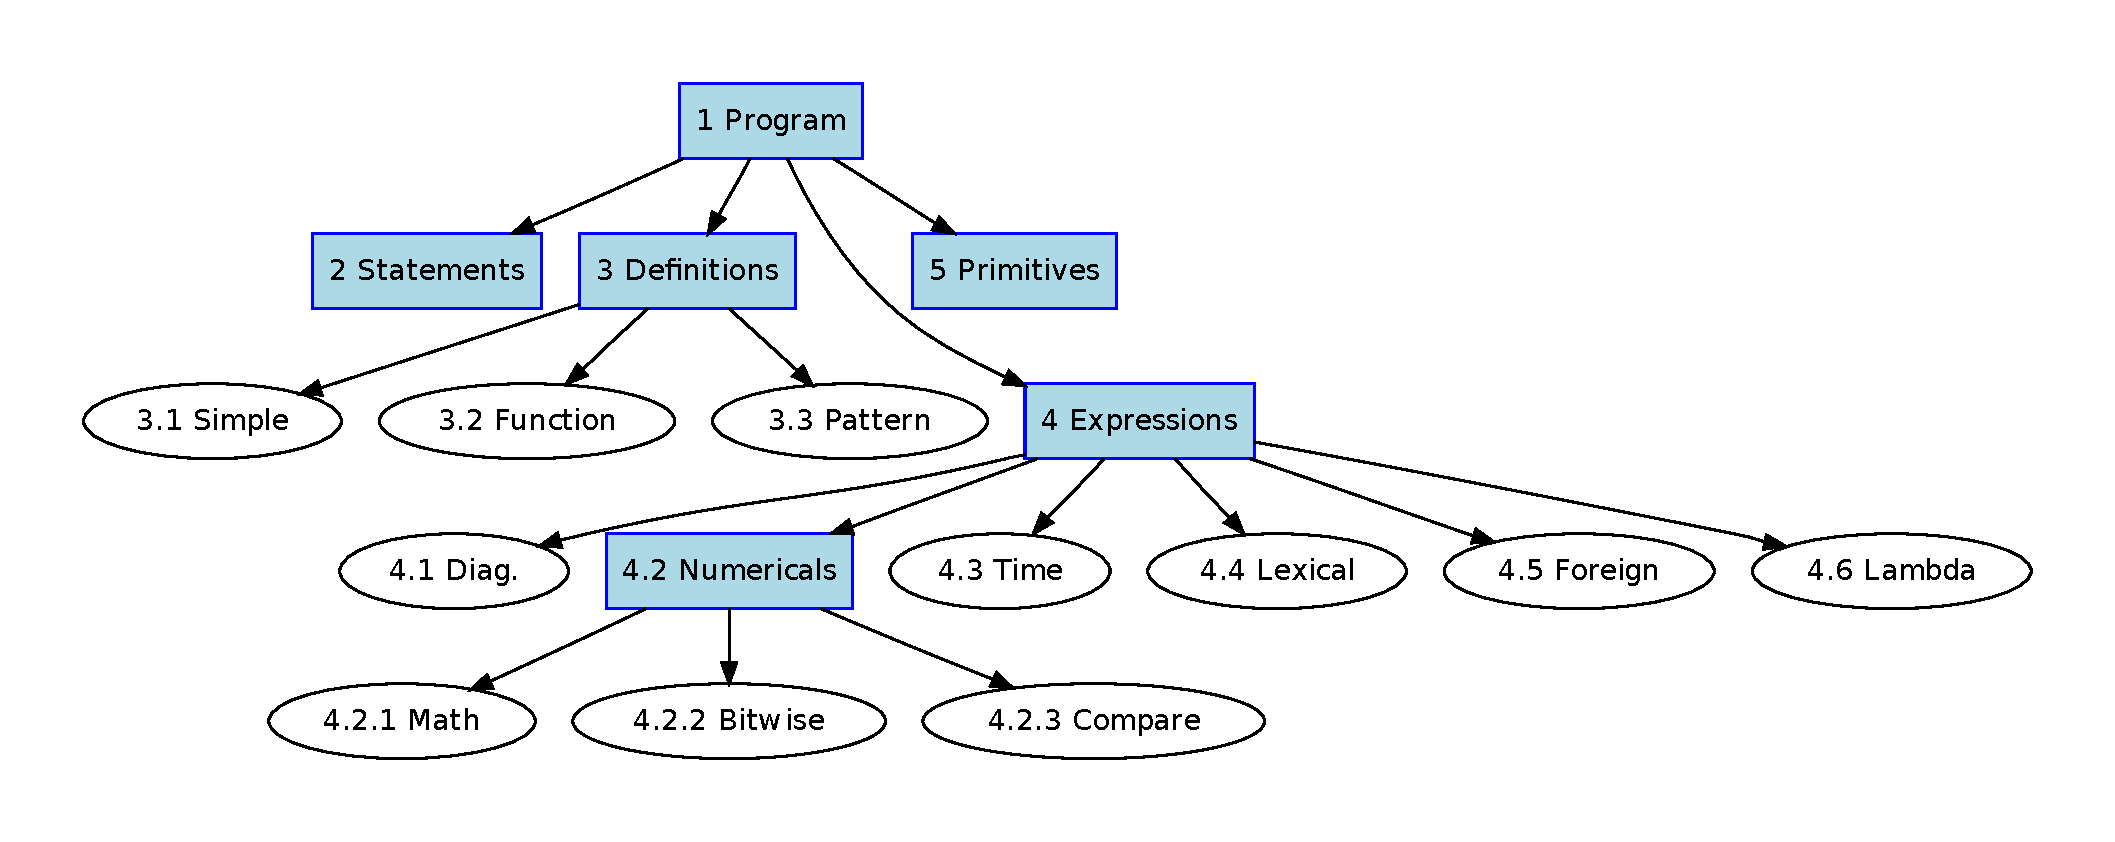
\includegraphics[scale=0.45]{illustrations/syntax-chart}
\caption{Overview of \faust syntax}
\label{fig:syntax}
\end{figure}

As we will see, \textit{definitions} and \textit{expressions} have a central role.

\section{\faust program}

A \faust program is essentially a list of \textit{statements}. These statements can be \textit{declarations}, \textit{imports} and \textit{definitions}, with optional C++ style (//... and /*...*/) comments.
 
\begin{grammar}
  <program> ::= 
  \begin{syntdiag}
    \begin{rep}
      <statement>
    \end{rep}
  \end{syntdiag}
\end{grammar}

Here is a short \faust program that implements of a simple noise generator. It exhibits the various kind of statements : two \textit{declarations}, an \textit{import}, a \textit{comment} and a \textit{definition}.

\begin{lstlisting}
declare name       "noise";
declare copyright  "(c)GRAME 2006";

import("music.lib");

// noise level controlled by a slider
process = noise * vslider("volume", 0, 0, 1, 0.1);
\end{lstlisting}
 
The keyword \lstinline'process' is the equivalent of \lstinline'main' in C/C++. Any \faust program, to be valid, must at least define \lstinline'process'.


\section{Statements}

The \textit{statements} of a \faust program are of three kinds : \textit{metadata declarations}, \textit{file imports} and \textit{definitions}. All statements end with a semicolon (\lstinline';'). 

\begin{grammar}
  <statement> ::= 
  \begin{syntdiag}
    \begin{stack}
      <declaration>\\
      <fileimport>\\
      <definition>
    \end{stack}
  \end{syntdiag}
\end{grammar}


\subsection{Declarations}

Meta-data declarations (for example \lstinline'declare name "noise";') are optional and typically used to document a \faust project. 

\begin{grammar}
  <declaration> ::= 
  \begin{syntdiag}
    "declare" <key> <string> ";"
  \end{syntdiag}
\end{grammar}

\begin{grammar}
  <key> ::= 
    <identifier>
\end{grammar}

Contrary to regular comments, these declarations will appear in the C++ code generated by the compiler.


\subsection{Imports}

File imports allow to import definitions from other source files.  

\begin{grammar}
  <fileimport> ::= 
  \begin{syntdiag}
    "import"  "(" <filename> ")" ";"
  \end{syntdiag}
\end{grammar}

For example \lstinline{import("math.lib");} imports the definitions of the \lstinline{math.lib} library, a set of additional mathematical functions provided as foreign functions.


\section{Definitions}

A \textit{definition} associates an identifier with an expression it stands for. 

Definitions are essentially a convenient shortcut avoiding to type long expressions. During compilation, more precisely during the evaluation stage, identifiers are replaced by their definitions. It is therefore always equivalent to use an identifier or directly its definition. Please note that multiple definitions of a same identifier are not allowed, unless it is a pattern matching based definition.

\subsection{Simple Definitions}

The syntax of a simple definition is:

\begin{grammar}
  <definition> ::= 
  \begin{syntdiag}
    <identifier> "=" <expression> ";"
  \end{syntdiag}
\end{grammar}

For example here is the definition of \lstinline'random', a simple pseudo-random number generator:

\begin{lstlisting}
 random = +(12345) ~ *(1103515245);
\end{lstlisting}


\subsection{Function Definitions}

Definitions with formal parameters correspond to functions definitions.


\begin{grammar}
  <definition> ::= 
  \begin{syntdiag}
    <identifier> "(" 
    \begin{rep}
      <parameter> \\ ","
    \end{rep}
    ")" "=" <expression> ";"
  \end{syntdiag}
\end{grammar}

For example the definition of \lstinline'linear2db', a function that converts linear values to decibels, is :

\begin{lstlisting}
 linear2db(x) = 20*log10(x);
\end{lstlisting}
 
Please note that this notation is only a convenient alternative to the direct use of \textit{lambda-abstractions} (also called anonymous functions). The following is an equivalent definition of \lstinline'linear2db' using a lambda-abstraction:

\begin{lstlisting}
 linear2db = \(x).(20*log10(x));
\end{lstlisting}


\subsection{Definitions with pattern matching}

Moreover, formal parameters can also be full expressions representing patterns. 

\begin{grammar}
  <definition> ::= 
  \begin{syntdiag}
    <identifier> "(" 
    \begin{rep}
      <pattern> \\ ","
    \end{rep}
    ")" "=" <expression> ";"
  \end{syntdiag}
\end{grammar}

\begin{grammar}
  <pattern> ::= 
    <identifier> |  <expression>
\end{grammar}

This powerful mechanism allows to algorithmically create and manipulate block diagrams expressions. Let's say that you want to describe a function to duplicate an expression several times in parallel:
\begin{lstlisting}
 duplicate(1,exp) = exp;
 duplicate(n,exp) = exp, duplicate(n-1,exp);
\end{lstlisting}

Please note that this last definition is a convenient alternative to the more verbose :
\begin{lstlisting}
 duplicate = case { 
               (1,exp) => exp; 
               (n,exp) => duplicate(n-1,exp); 
             };
\end{lstlisting}

 
  
\section{Expressions}

Despite its textual syntax, \faust is conceptually a block-diagram language. \faust expressions represent DSP block-diagrams and are assembled from primitive ones using various \textit{composition} operations. More traditional \textit{numerical} expressions in infix notation are also possible. Additionally \faust provides time based expressions, like delays, expressions related to lexical environments, expressions to interface with foreign function and lambda expressions.

\begin{grammar}
  <expression> ::= 
  \begin{syntdiag}
    \begin{stack}
      <diagram>\\
      <numerical>\\
      <time>\\
      <lexical>\\
      <foreign>\\
      <lambda>
    \end{stack}
  \end{syntdiag}
\end{grammar}
  
\subsection{Diagram Expressions}

Diagram expressions are assembled from primitive ones using either binary composition operations or high level iterative constructions.
 
\begin{grammar}
  <diagramexp> ::= 
  \begin{syntdiag}
    \begin{stack}
      <diagcomposition>\\
      <diagiteration>
    \end{stack}
  \end{syntdiag}
\end{grammar}

\subsubsection{Diagram composition operations} 
Five binary composition operations are available to combine block-diagrams : \textit{recursion}, \textit{parallel}, \textit{sequential}, \textit{split} and \textit{merge} composition.

\begin{grammar}
  <diagcomposition> ::= 
  \begin{syntdiag}
    <expression>
    \begin{stack}
      "~" \\ "," \\ ":" \\ "<:" \\ ":>"
    \end{stack}
    <expression>
  \end{syntdiag}
\end{grammar}

Among these operations, recursion (\lstinline'~') has the highest priority and split (\lstinline'<:') and merge (\lstinline':>') the lowest (see table \ref{table:composition}).
 
\begin{table}[ht]
	\centering
	\begin{tabular}{|l|l|l|}
		\hline
		\textbf{Syntax} & \textbf{Pri.}  & \textbf{Description} \\
		\hline
		\texttt{\farg{expression}\ $\sim$\ \farg{expression}}		& 4 & recursive composition     \\
		\texttt{\farg{expression}\ ,\ \farg{expression}}			& 3 & parallel composition      \\
		\texttt{\farg{expression}\ :\ \farg{expression}}			& 2 & sequential composition    \\
		\texttt{\farg{expression}\ <:\ \farg{expression}}			& 1 & split composition      	\\
		\texttt{\farg{expression}\ :>\ \farg{expression}}			& 1 & merge composition      	\\
		\hline
	\end{tabular}
	\caption{Block-Diagram composition operation priorities}   
  	\label{table:composition}
\end{table}
 


\paragraph{Parallel Composition}
The \emph{parallel composition}  \lstinline$A,B$ (figure \ref{figure:par1}) is probably the simplest one. It places the two block-dia\-grams one on top of the other, without connections. The inputs of the resulting block-diagram are the inputs of \lstinline$A$ and \lstinline$B$. The outputs of the resulting block-diagram are the outputs of \lstinline$A$ and \lstinline$B$.

\begin{figure}[h]
\centering
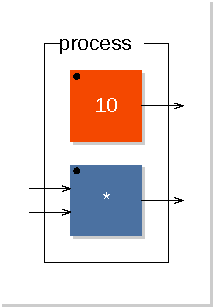
\includegraphics[scale=0.7]{images/par1}
\caption{Example of parallel composition  \lstinline'(10,*)'}
\label{figure:par1}
\end{figure}


\paragraph{Sequential Composition}
The \emph{sequential composition}  \lstinline$A:B$ (figure \ref{figure:seq1}) connects the outputs of  $A$ to the inputs of  $B$.  $A[0]$ is connected to $[0]B$,   $A[1]$ is connected to $[1]B$, and so on. 

\begin{figure}[h]
\centering 
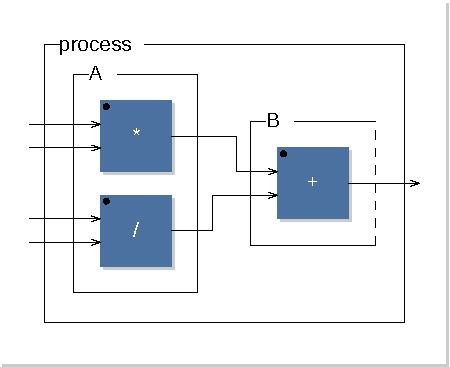
\includegraphics[scale=0.7]{images/seq1}
\caption{Example of sequential composition  \lstinline'((*,/):+)' } 
\label{figure:seq1}
\end{figure}


\paragraph{Split Composition}
The \emph{split composition}  \lstinline$A<:B$ (figure \ref{figure:split1}) operator is used to distribute the outputs
of $A$ to the inputs of $B$

\begin{figure}[h]
\centering 
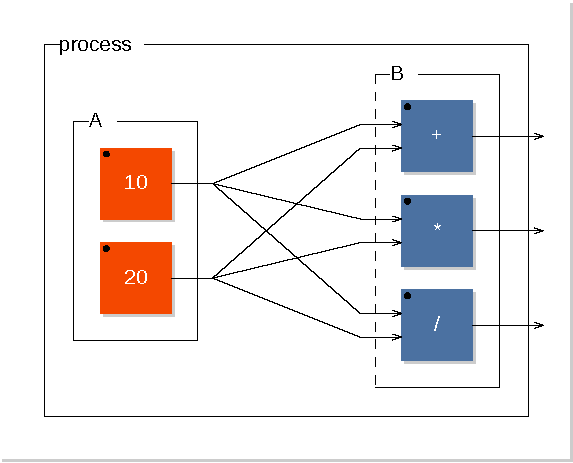
\includegraphics[scale=0.7]{images/split1} 
\caption{example of split composition   \lstinline'((10,20) <: (+,*,/))'}  
\label{figure:split1}
\end{figure}


\paragraph{Merge Composition}
The \emph{merge composition}  \lstinline$A:>B$ (figure \ref{figure:merge1})is used to connect several outputs
of  $A$ to the same inputs of $B$. 

\begin{figure}[h]
\centering 
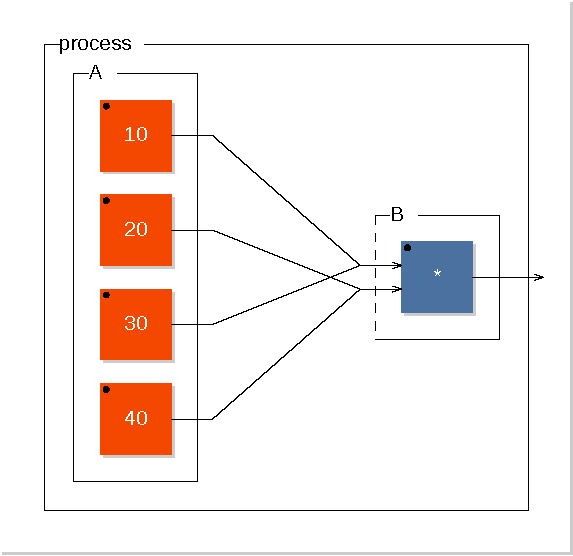
\includegraphics[scale=0.7]{images/merge1} 
\caption{example of merge composition \lstinline'((10,20,30,40) :> *)'}  
\label{figure:merge1}
\end{figure}
 

\paragraph{Recursive Composition}
    The \emph{recursive composition} \lstinline'A~B' (figure \ref{figure:rec1})is used to create cycles in the block-diagram in order to express recursive computations.
    
    \begin{figure}[h]
    \centering 
    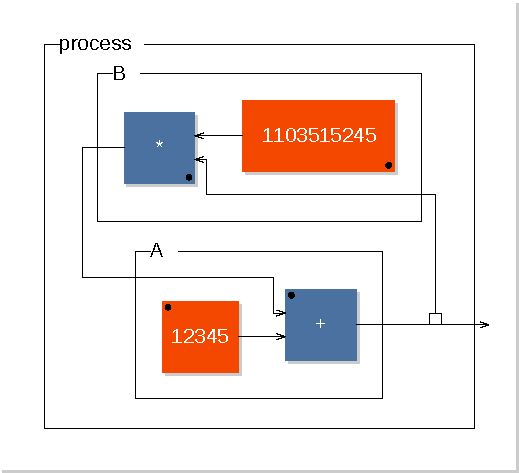
\includegraphics[scale=0.7]{images/rec1} 
    \caption{example of recursive composition \lstinline'+(12345) ~ *(1103515245)'}  
    \label{figure:rec1}
    \end{figure}
 


%Let's see these composition operations in action with two simple examples (figure \ref{fig:integrator}). 

%The first example uses the recursive composition operator (\lstinline'~'). It is an integrator \lstinline'process = +~_;' that produces an output signal $Y$ such that $Y(t)=X(t)+Y(t-1)$.

%\begin{figure}[t]
%  \centering
%  \begin{tabular}{ccc}
%    \includegraphics[scale=0.7]{illustrations/integrator}&
%    \includegraphics[scale=0.7]{illustrations/ms}
%  \end{tabular}
%  \caption{a) integrator, b) mid/side stereo matrix}   
%  \label{fig:integrator}
%\end{figure}


%The second example uses the parallel (\lstinline',') and split (\lstinline'<:') composition operators. It implements a Mid/Side stereophonic matrix: \lstinline'process = _,_<:+,-;' that produces two output signals $Y_0$ and $Y_1$ such that $Y_0(t)=X_0(t)+X_1(t)$ and $Y_1(t)=X_0(t)-X_1(t)$

 
\subsubsection{Iterations} 
Iterations are analog to \lstinline'for(...)' loops and provide a convenient way to automate some complex block-diagram constructions. 

\begin{grammar}
  <diagiteration> ::= 
  \begin{syntdiag}
    \begin{stack}
       "par" "(" <ident> "," <numiter> "," <expression> ")"\\
      "seq" "(" <ident> "," <numiter> "," <expression> ")"\\
      "sum" "(" <ident> "," <numiter> "," <expression> ")"\\
      "prod" "(" <ident> "," <numiter> "," <expression> ")"
    \end{stack}
  \end{syntdiag}
\end{grammar}

The following example shows the usage of  \lstinline'seq' to create a 10-bands filter:

\begin{lstlisting}
process  =	seq(i, 10, 
				vgroup("band %i", 
					bandfilter( 1000*(1+i) ) 
				) 
			);
\end{lstlisting}

       
\begin{grammar}
  <numiter> ::= <expression>
\end{grammar}

The number of iterations must be a constant expression. 


\subsection{Numerical Expressions}

Numerical expressions are essentially syntactic sugar allowing to use a familiar infix notation to express mathematical expressions, bitwise operations and to compare signals. Please note that is this section only built-in primitives with an infix syntax are presented. A complete description of all the build-ins is available in the primitive section (see \ref{primitives}). 

\begin{grammar}
  <numerical> ::= 
  \begin{syntdiag}
    \begin{stack}
      <math>\\
      <bitwise>\\
      <comparison>
    \end{stack}
  \end{syntdiag}
\end{grammar}

\subsubsection{Mathematical expressions} are the familiar 4 operations as well as the modulo and power operations

\begin{grammar}
  <math> ::= 
  \begin{syntdiag}
    <expression>
    \begin{stack}
      "+" \\ "-" \\ "*" \\ "/" \\ "\%" \\ "^"
    \end{stack}
    <expression>
  \end{syntdiag}
\end{grammar}

\subsubsection{Bitwise expressions} are the boolean operations and the left and right arithmetic shifts.

\begin{grammar}
  <bitwise> ::= 
  \begin{syntdiag}
    <expression>
    \begin{stack}
      "|" \\ "\&" \\ "xor" \\ "<<" \\ ">>"
    \end{stack}
    <expression>
  \end{syntdiag}
\end{grammar}

\subsubsection{Comparison} operations allow to compare signals and result in a boolean signal that is 1 when the condition is true and 0 when the condition is false.

\begin{grammar}
  <bitwise> ::= 
  \begin{syntdiag}
    <expression>
    \begin{stack}
      "<" \\ "<=" \\ ">" \\ ">=" \\ "==" \\ "!="
    \end{stack}
    <expression>
  \end{syntdiag}
\end{grammar}


\subsection{Time expressions}

Time expressions are used to express delays. The notation \lstinline'X@10' represent the signal \lstinline'X' delayed by 10 samples. The notation \lstinline"X'" represent the signal X delayed by one sample and is therefore equivalent to \lstinline'X@1'.

\begin{grammar}
  <time> ::= 
  \begin{syntdiag}
    \begin{stack}
      <expression> "@" <expression> \\ 
      <expression> "'"
    \end{stack}
  \end{syntdiag}
\end{grammar}

The delay don't have to be fixed, but it must be positive and bounded. The values of a slider are perfectcly acceptable as in the following example:

\begin{lstlisting}
process = @(hslider("delay",0, 0, 100, 1));
\end{lstlisting}

\subsection{Environment expressions}
Each \faust expression has an associated lexical environment : a list of dictionaries where to look for definitions. The following expressions allow to create and access such environments.

\begin{grammar}
  <envexp> ::= 
  \begin{syntdiag}
    \begin{stack}
      <expression> "with" "\{"
        \begin{rep}
          <defintion>
        \end{rep}
        "\}" \\ 
      "environment" "\{"
        \begin{rep}
          <defintion>
        \end{rep}
        "\}" \\ 
      <expression> "." <ident> \\
      "library" "(" <filename> ")" \\
      "component" "(" <filename> ")"
    \end{stack}
  \end{syntdiag}
\end{grammar}

\subsubsection{With expression}allows to specify a \textit{local environment}, a private list of definition that will be used to evaluate the left hand expression

\begin{grammar}
  <withexpression> ::= 
  \begin{syntdiag}
      <expression> "with" "\{"
        \begin{rep}
          <defintion>
        \end{rep}
        "\}"
  \end{syntdiag}
\end{grammar}

In the following example :
\begin{lstlisting}
pink = f : + ~ g with {
	f(x) = 0.04957526213389*x 
		 - 0.06305581334498*x' 
         + 0.01483220320740*x'';
	g(x) = 1.80116083982126*x 
		 - 0.80257737639225*x';
};
\end{lstlisting}
the definitions of \lstinline'f(x)' and \lstinline'g(x)' are local to the expression \lstinline'f : + ~ g':

\subsubsection{Environment expression} allows to create an explicit environment: like a \lstinline'with', but without a left hand expression. It is a convenient way to group together related definitions, to isolate groups of definitions and to create a name space hierarchy. 

\begin{grammar}
  <environment> ::= 
  \begin{syntdiag}
      "environment" "\{"
        \begin{rep}
          <defintion>
        \end{rep}
        "\}"
  \end{syntdiag}
\end{grammar}

In the following example an environment is used to group together some constant definitions :

\begin{lstlisting}
constant = environment {
	pi = 3.14159;
	e = 2,718 ;
	...
};
\end{lstlisting}

\subsubsection{Access} Definitions inside an environment can be accessed using 
the '.' construction. 

\begin{grammar}
  <access> ::= 
  \begin{syntdiag}
      <expression> "." <ident>
  \end{syntdiag}
\end{grammar}

For example \lstinline'constant.pi' refers to the definition of \lstinline'pi' in the environment above.

Please note that environment don't have to be named. We could have written directly 
\lstinline'environment{pi = 3.14159; e = 2,718;....}.pi'



\subsubsection{Library} allows to create an environment by reading the definitions from a file.

\begin{grammar}
  <library> ::= 
  \begin{syntdiag}
      "library" "(" <filename> ")"
  \end{syntdiag}
\end{grammar}

For example \lstinline'library("filter.lib")' represents the lexical environment 
obtained by reading the file "filter.lib". It works like \lstinline'import("filter.lib")' but all the read definitions are stored in a new separate lexical environment.


\subsubsection{Component} is a powerful construction that allows to reuse a full \faust program as a simple expression.

\begin{grammar}
  <component> ::= 
  \begin{syntdiag}
    "component" "(" <filename> ")"
  \end{syntdiag}
\end{grammar}

 For example \lstinline'component("freeverb.dsp")' denotes the signal processor defined in file "freeverb.dsp". 
 
 Components can be used within expressions like in: 
 \begin{lstlisting}
 ...component("karplus32.dsp"):component("freeverb.dsp")... 
 \end{lstlisting}
 
 Please note that \lstinline'component("freeverb.dsp")' is equivalent to \lstinline'library("freeverb.dsp").process'.


\subsection{Foreign expressions}

Reference to external C \textit{functions}, \textit{variables} and \textit{constants} can be introduced using the \textit{foreign function} mechanism.

\begin{grammar}
  <foreignexp> ::= 
  \begin{syntdiag}
    \begin{stack}
      "ffunction" "(" <signature> "," <includefile> "," <comment> ")" \\
      "fvariable" "(" <type> <identifier> "," <includefile> ")" \\
      "fconstant" "(" <type> <identifier> "," <includefile> ")" 
    \end{stack}
  \end{syntdiag}
\end{grammar}


\subsubsection{function} An external C function is declared by indicating its name and signature as well as the required include file.
The file \lstinline'"math.lib"' of the \faust distribution contains several foreign function definitions, for example the inverse hyperbolic sine function \lstinline'asinh':

\begin{lstlisting}
asinh = ffunction(float asinhf (float), <math.h>, "");
\end{lstlisting}

Foreign functions with input parameters are considered pure math functions. They are therefore considered free of side effects and called only when their parameters change (that is at the rate of the fastest parameter). 

Exceptions are functions with no input parameters. A typical example is the C \lstinline'rand()' function. In this case the compiler generate code to call the function at sample rate.


\subsubsection{signature} 
The signature part (\lstinline'float asinhf (float)' in our previous example) describes the prototype of the C function : return type, function name and list of parameter types. 

\begin{grammar}
  <signature> ::= 
  \begin{syntdiag}
    <type> <identifier> "("
    \begin{rep}
      <type> \\ ","
    \end{rep}
    ")"
  \end{syntdiag}
\end{grammar}

\subsubsection{types}
Note that currently only numerical functions involving simple int and float parameters are allowed. No vectors, tables or data structures can be passed as parameters or returned.

\begin{grammar}
  <type> ::= 
      <int> | <float>
\end{grammar}

% \begin{grammar}
%   <type> ::= 
%   \begin{syntdiag}
%     \begin{stack}
%       "int" \\ "float"
%     \end{stack}
%   \end{syntdiag}
% \end{grammar}

\subsubsection{variables and constants} 
External variables and constants can also be declared with a similar syntax. In the same \lstinline'"math.lib"' file we can found the definition of the sampling rate constant \lstinline'SR' and the definition of the block-size variable \lstinline'BS' :

\begin{lstlisting}
SR 			= fconstant(int fSamplingFreq, <math.h>);
BS          = fvariable(int count, <math.h>);
\end{lstlisting}

Foreign constants are not supposed to vary. Therefore expressions involving only foreign constants are only computed once, during the initialization period. 

Variable are considered to vary at block speed. This means that expressions depending of external variables are computed every block.


\subsubsection{include file}
In declaring foreign functions one as also to specify the include file. It allows the \faust compiler to add the corresponding \lstinline'#include...' in the generated code.

\begin{grammar}
  <includefile> ::= 
  \begin{syntdiag}
    \begin{stack}
      "<"
      \begin{rep}
        <char>
      \end{rep}
      ">" \\ 
      "\""
      \begin{rep}
        <char>
      \end{rep}
      "\""
    \end{stack}
  \end{syntdiag}
\end{grammar}


%The syntax of these foreign declarations is the following :
%The foreign function mechanism allows to use external functions, variables and constants. External functions are limited to numerical ones. 
%  

%\begin{lstlisting}
%process = ffunction(float toto (), "foo.h", "commentaire");
%\end{lstlisting}


%ffunction are pure math unless no params
%difference between fconstant and fvariable

%\begin{lstlisting}
%SR 			= fconstant(int fSamplingFreq, <math.h>);
%BS          = fvariable(int count, <math.h>);
%\end{lstlisting}

%\begin{rail}
%includefile : '<' (char+) '>' | string;

%signature : type identifier '(' (type + ',') ')';

%type : 'int'|'float';
%\end{rail}

%that take simple numerical parameters and return a number.
%Foreign functions, variables and constants. Example of foreign function expression : \lstinline'ffunction (float acoshf (float), <math.h>, "")'.

\subsection{Applications and Abstractions}

\textit{Abstractions} and \textit{applications} are fundamental programming constructions directly inspired by the Lambda-Calculus. These constructions provide powerful ways to describe and transform block-diagrams algorithmically.

\begin{grammar}
  <progexp> ::= 
  \begin{syntdiag}
    \begin{stack}
      <abstraction> \\ <application>
    \end{stack}
  \end{syntdiag}
\end{grammar}

\subsubsection{Abstractions}

Abstractions correspond to functions definitions and allow to generalize a block-diagram by \textit{making variable} some of its parts. 

\begin{grammar}
  <abstraction> ::= 
  \begin{syntdiag}
    \begin{stack}
      <lambdaabstraction> \\ <patternabstraction>
    \end{stack}
  \end{syntdiag}
\end{grammar}

\begin{grammar}
  <lambdaabstraction> ::= 
  \begin{syntdiag}
    "\\" "(" 
    \begin{rep}
      <ident> \\ ","
    \end{rep}
    ")" "." "(" <expression> ")"
  \end{syntdiag}
\end{grammar}

Let's say you want to transform a stereo reverb, \lstinline'freeverb' for instance, into a mono effect. You can write the following expression: 
\begin{lstlisting}
	_ <: freeverb :> _ 
\end{lstlisting}
The incoming mono signal is splitted to feed the two input channels of the reverb, while the two output channels of the reverb are mixed together to produce the resulting mono output.

Imagine now that you are interested in transforming other stereo effects. It can be interesting to generalize this principle by making \lstinline'freeverb' a variable: 
\begin{lstlisting}
	\(freeverb).(_ <: freeverb :> _)
\end{lstlisting}

The resulting abstraction can then be applied to transform other effects. Note that if \lstinline'freeverb' is a perfectly valid variable name, a more neutral name would probably be easier to read like:
\begin{lstlisting}
	\(fx).(_ <: fx :> _)
\end{lstlisting}
 
Moreover it could be convenient to give a name to this abstraction:
\begin{lstlisting}
	mono = \(fx).(_ <: fx :> _);
\end{lstlisting}

Or even use a more traditional, but equivalent, notation:
\begin{lstlisting}
	mono(fx) = _ <: fx :> _;
\end{lstlisting}


\subsubsection{Applications}
Applications correspond to function calls and allow to replace the variable parts of an abstraction with the specified arguments.

\begin{grammar}
  <application> ::= 
  \begin{syntdiag}
    <expression> "(" 
    \begin{rep}
      <expression> \\ ","
    \end{rep}
    ")"
  \end{syntdiag}
\end{grammar}

For example you can apply the previous abstraction to transform your stereo harmonizer:
\begin{lstlisting}
	mono(harmonizer)
\end{lstlisting}

The compiler will start by replacing \lstinline'mono' by its definition:
\begin{lstlisting}
	\(fx).(_ <: fx :> _)(harmonizer)
\end{lstlisting}

Whenever the \faust compiler find an application of an abstraction it replaces the variable part with the argument \footnote{This is called $\beta$-reduction in Lambda-Calculus}. The resulting expression is as expected:
\begin{lstlisting}
	(_ <: harmonizer :> _)
\end{lstlisting}



\subsubsection{Pattern Matching}
Pattern matching rules provide an effective way to analyze and transform block-diagrams algorithmically.

\begin{grammar}
  <patternabstraction> ::= 
  \begin{syntdiag} 
    "case" "\{"
    \begin{rep}
      <rule>
    \end{rep}
    "\}"
  \end{syntdiag}
\end{grammar}

\begin{grammar}
  <rule> ::= 
  \begin{syntdiag} 
    "("
    \begin{rep}
      <pattern> \\ ","
    \end{rep}
    ")" "=>" <expression> ";"
  \end{syntdiag}
\end{grammar}

\begin{grammar}
  <pattern> ::= 
    <ident> | <expression>
\end{grammar}

% \begin{grammar}
%   <pattern> ::= 
%   \begin{syntdiag} 
%     \begin{stack}
%     <ident> \\
%     <expression>
%     \end{stack}
%   \end{syntdiag}
% \end{grammar}

For example \lstinline'case{ (x:y) => y:x; (x) => x; }' contains two rules. The first one will match a sequential expression and invert the two part. The second one will match all remaining expressions and leave it untouched. Therefore the application:

\begin{lstlisting}
	case{(x:y) => y:x; (x) => x;}(freeverb:harmonizer)
\end{lstlisting}

will produce:

\begin{lstlisting}
	(harmonizer:freeverb)
\end{lstlisting}

Please note that patterns are evaluated before the pattern matching operation. Therefore only variables that appear free in the pattern are binding variables during pattern matching. 



%--------------------------------------------------------------------------------------------------------------
\section{Primitives}
%--------------------------------------------------------------------------------------------------------------
\label{primitives}
The primitive signal processing operations represent the built-in functionalities of \faust, that is the atomic operations on signals provided by the language. All these primitives denote \emph{signal processors}, functions transforming \emph{input signals} into \emph{output signals}.

%--------------------------------------------------------------------------------------------------------------
\subsection{Numbers}
%--------------------------------------------------------------------------------------------------------------

\faust considers two types of numbers : \textit{integers} and \textit{floats}. Integers are implemented as 32-bits integers, and floats are implemented either with a simple, double or extended precision depending of the compiler options.

\begin{grammar}
  <int> ::= 
  \begin{syntdiag}
    \begin{stack}
      \\ "+" \\ "-"
    \end{stack}
    \begin{rep}
      <digit>
    \end{rep}
  \end{syntdiag}
\end{grammar}

\begin{grammar}
  <float> ::= 
  \begin{syntdiag}
    \begin{stack}
      \\ "+" \\ "-"
    \end{stack}
    \begin{stack}
      \begin{rep}<digit>\end{rep} "." \begin{stack} \begin{rep}<digit>\end{rep} \\ \end{stack} \\
      \begin{stack} \begin{rep}<digit>\end{rep} \\ \end{stack} "." \begin{rep}<digit>\end{rep}
    \end{stack}
  \end{syntdiag}
\end{grammar}

\begin{grammar}
  <digit> ::= 
  0 | 1 | 2 | 3 | 4 | 5 | 6 | 7 | 8 | 9
\end{grammar}


\bigskip

Like any other \faust expression, numbers are signal processors. For example the number $0.95$ is a signal processor of type $\mathbb{S}^{0}\rightarrow\mathbb{S}^{1}$ that transforms an empty tuple of signals $()$ into a 1-tuple of signals $(y)$ such that $\forall t\in\mathbb{N}, y(t)=0.95$.

%\begin{tabular}{|l|l|l|}
%\hline
%\textbf{Syntax} & \textbf{Type}  & \textbf{Description} \\
%\hline
%$n$ & $\mathbb{S}^{0}\rightarrow\mathbb{S}^{1}$ & integer number: $y(t)=n$ \\
%$r$ & $\mathbb{S}^{0}\rightarrow\mathbb{S}^{1}$ & floating point number: $y(t)=r$ \\
%\hline

%\end{tabular}

%--------------------------------------------------------------------------------------------------------------
\subsection{C-equivalent primitives}
%--------------------------------------------------------------------------------------------------------------

Most \faust primitives are analogue to their C counterpart but lifted to signal processing.
For example $+$ is a function of type $\mathbb{S}^{2}\rightarrow\mathbb{S}^{1}$ that transforms a pair of signals $(x_1,x_2)$ into a 1-tuple of signals $(y)$ such that $\forall t\in\mathbb{N}, y(t)=x_{1}(t)+x_{2}(t)$.

\bigskip

\begin{tabular}{|l|l|l|}
\hline
\textbf{Syntax} & \textbf{Type}  & \textbf{Description} \\
\hline
$n$ & $\mathbb{S}^{0}\rightarrow\mathbb{S}^{1}$ & integer number: $y(t)=n$ \\
$n.m$ & $\mathbb{S}^{0}\rightarrow\mathbb{S}^{1}$ & floating point number: $y(t)=n.m$ \\

\texttt{\_} & $\mathbb{S}^{1}\rightarrow\mathbb{S}^{1}$ & identity function: $y(t)=x(t)$ \\
\texttt{!} & $\mathbb{S}^{1}\rightarrow\mathbb{S}^{0}$ & cut function: $\forall x\in\mathbb{S},(x)\rightarrow ()$\\

\texttt{int} & $\mathbb{S}^{1}\rightarrow\mathbb{S}^{1}$ & cast into an int signal: $y(t)=(int)x(t)$  \\
\texttt{float} & $\mathbb{S}^{1}\rightarrow\mathbb{S}^{1}$ & cast into an float signal: $y(t)=(float)x(t)$  \\

\texttt{+} & $\mathbb{S}^{2}\rightarrow\mathbb{S}^{1}$ & addition: $y(t)=x_{1}(t)+x_{2}(t)$  \\
\texttt{-} & $\mathbb{S}^{2}\rightarrow\mathbb{S}^{1}$ & subtraction: $y(t)=x_{1}(t)-x_{2}(t)$   \\
\texttt{*} & $\mathbb{S}^{2}\rightarrow\mathbb{S}^{1}$ & multiplication: $y(t)=x_{1}(t)*x_{2}(t)$   \\
\texttt{$\land$} & $\mathbb{S}^{2}\rightarrow\mathbb{S}^{1}$ & power: $y(t)=x_{1}(t)^{x_{2}(t)}$   \\
\texttt{/} & $\mathbb{S}^{2}\rightarrow\mathbb{S}^{1}$ & division: $y(t)=x_{1}(t)/x_{2}(t)$   \\
\texttt{\%} & $\mathbb{S}^{2}\rightarrow\mathbb{S}^{1}$ & modulo: $y(t)=x_{1}(t)\%x_{2}(t)$   \\

\texttt{\&} & $\mathbb{S}^{2}\rightarrow\mathbb{S}^{1}$ & logical AND: $y(t)=x_{1}(t)\&x_{2}(t)$   \\
\texttt{|} & $\mathbb{S}^{2}\rightarrow\mathbb{S}^{1}$ & logical OR: $y(t)=x_{1}(t)|x_{2}(t)$   \\
\texttt{xor} & $\mathbb{S}^{2}\rightarrow\mathbb{S}^{1}$ & logical XOR: $y(t)=x_{1}(t)\land x_{2}(t)$   \\

\texttt{<<} & $\mathbb{S}^{2}\rightarrow\mathbb{S}^{1}$ & arith. shift left: $y(t)=x_{1}(t) << x_{2}(t)$   \\
\texttt{>>} & $\mathbb{S}^{2}\rightarrow\mathbb{S}^{1}$ & arith. shift right: $y(t)=x_{1}(t) >> x_{2}(t)$   \\


\texttt{<} & $\mathbb{S}^{2}\rightarrow\mathbb{S}^{1}$ & less than: $y(t)=x_{1}(t) < x_{2}(t)$   \\
\texttt{<=} & $\mathbb{S}^{2}\rightarrow\mathbb{S}^{1}$ & less or equal: $y(t)=x_{1}(t) <= x_{2}(t)$   \\
\texttt{>} & $\mathbb{S}^{2}\rightarrow\mathbb{S}^{1}$ & greater than: $y(t)=x_{1}(t) > x_{2}(t)$   \\
\texttt{>=} & $\mathbb{S}^{2}\rightarrow\mathbb{S}^{1}$ & greater or equal: $y(t)=x_{1}(t) >= x_{2}(t)$   \\
\texttt{==} & $\mathbb{S}^{2}\rightarrow\mathbb{S}^{1}$ & equal: $y(t)=x_{1}(t) == x_{2}(t)$   \\
\texttt{!=} & $\mathbb{S}^{2}\rightarrow\mathbb{S}^{1}$ & different: $y(t)=x_{1}(t) != x_{2}(t)$   \\

\hline

\end{tabular}

\bigskip


%--------------------------------------------------------------------------------------------------------------
\subsection{\texttt{math.h}-equivalent primitives}
%--------------------------------------------------------------------------------------------------------------

Most of the C \texttt{math.h} functions are also built-in as primitives (the others are defined as external functions in file \texttt{math.lib}).

\bigskip
\begin{tabular}{|l|l|l|}
\hline
\textbf{Syntax} & \textbf{Type}  & \textbf{Description} \\
\hline

\texttt{acos} & $\mathbb{S}^{1}\rightarrow\mathbb{S}^{1}$ & arc cosine: $y(t)=\mathrm{acosf}(x(t))$ \\
\texttt{asin} & $\mathbb{S}^{1}\rightarrow\mathbb{S}^{1}$ & arc sine: $y(t)=\mathrm{asinf}(x(t))$ \\
\texttt{atan} & $\mathbb{S}^{1}\rightarrow\mathbb{S}^{1}$ & arc tangent: $y(t)=\mathrm{atanf}(x(t))$ \\
\texttt{atan2} & $\mathbb{S}^{2}\rightarrow\mathbb{S}^{1}$ & arc tangent of 2 signals: $y(t)=\mathrm{atan2f}(x_{1}(t), x_{2}(t))$ \\

\texttt{cos} & $\mathbb{S}^{1}\rightarrow\mathbb{S}^{1}$ & cosine: $y(t)=\mathrm{cosf}(x(t))$ \\
\texttt{sin} & $\mathbb{S}^{1}\rightarrow\mathbb{S}^{1}$ & sine: $y(t)=\mathrm{sinf}(x(t))$ \\
\texttt{tan} & $\mathbb{S}^{1}\rightarrow\mathbb{S}^{1}$ & tangent: $y(t)=\mathrm{tanf}(x(t))$ \\

\texttt{exp} & $\mathbb{S}^{1}\rightarrow\mathbb{S}^{1}$ & base-e exponential: $y(t)=\mathrm{expf}(x(t))$ \\
\texttt{log} & $\mathbb{S}^{1}\rightarrow\mathbb{S}^{1}$ & base-e logarithm: $y(t)=\mathrm{logf}(x(t))$ \\
\texttt{log10} & $\mathbb{S}^{1}\rightarrow\mathbb{S}^{1}$ & base-10 logarithm: $y(t)=\mathrm{log10f}(x(t))$ \\
\texttt{pow} & $\mathbb{S}^{2}\rightarrow\mathbb{S}^{1}$ & power: $y(t)=\mathrm{powf}(x_{1}(t),x_{2}(t))$ \\
\texttt{sqrt} & $\mathbb{S}^{1}\rightarrow\mathbb{S}^{1}$ & square root: $y(t)=\mathrm{sqrtf}(x(t))$ \\
\texttt{abs} & $\mathbb{S}^{1}\rightarrow\mathbb{S}^{1}$ & absolute value (int): $y(t)=\mathrm{abs}(x(t))$ \\
			&											 & absolute value (float): $y(t)=\mathrm{fabsf}(x(t))$ \\
\texttt{min} & $\mathbb{S}^{2}\rightarrow\mathbb{S}^{1}$ & minimum: $y(t)=\mathrm{min}(x_{1}(t),x_{2}(t))$ \\
\texttt{max} & $\mathbb{S}^{2}\rightarrow\mathbb{S}^{1}$ & maximum: $y(t)=\mathrm{max}(x_{1}(t),x_{2}(t))$ \\
\texttt{fmod} & $\mathbb{S}^{2}\rightarrow\mathbb{S}^{1}$ & float modulo: $y(t)=\mathrm{fmodf}(x_{1}(t),x_{2}(t))$ \\
\texttt{remainder} & $\mathbb{S}^{2}\rightarrow\mathbb{S}^{1}$ & float remainder: $y(t)=\mathrm{remainderf}(x_{1}(t),x_{2}(t))$ \\

\texttt{floor} & $\mathbb{S}^{1}\rightarrow\mathbb{S}^{1}$ & largest int $\leq$: $y(t)=\mathrm{floorf}(x(t))$ \\
\texttt{ceil} & $\mathbb{S}^{1}\rightarrow\mathbb{S}^{1}$ & smallest int $\geq$: $y(t)=\mathrm{ceilf}(x(t))$ \\
\texttt{rint} & $\mathbb{S}^{1}\rightarrow\mathbb{S}^{1}$ & closest int: $y(t)=\mathrm{rintf}(x(t))$ \\

\hline
\end{tabular}
\bigskip





%--------------------------------------------------------------------------------------------------------------
\subsection{Delay, Table, Selector primitives}
%--------------------------------------------------------------------------------------------------------------

The following primitives allow to define fixed delays, read-only and read-write tables and 2 or 3-ways selectors (see figure \ref{fig:delays}).

\bigskip
\begin{tabular}{|l|l|l|}
\hline
\textbf{Syntax} & \textbf{Type}  & \textbf{Description} \\
\hline

\texttt{mem} & $\mathbb{S}^{1}\rightarrow\mathbb{S}^{1}$ 		& 1-sample delay: 	$y(t+1)=x(t),y(0)=0$  \\
\texttt{prefix} & $\mathbb{S}^{2}\rightarrow\mathbb{S}^{1}$ 	& 1-sample delay:  	$y(t+1)=x_{2}(t),y(0)=x_{1}(0)$  \\
\texttt{@} & $\mathbb{S}^{2}\rightarrow\mathbb{S}^{1}$ 			& fixed delay:  	$y(t+x_{2}(t))=x_{1}(t), y(t<x_{2}(t))=0$  \\

\texttt{rdtable} & $\mathbb{S}^{3}\rightarrow\mathbb{S}^{1}$ 	& read-only table:	$y(t)=T[r(t)]$  \\
\texttt{rwtable} & $\mathbb{S}^{5}\rightarrow\mathbb{S}^{1}$ 	& read-write table:	$T[w(t)]=c(t); y(t)=T[r(t)]$  \\

\texttt{select2} & $\mathbb{S}^{3}\rightarrow\mathbb{S}^{1}$ 	& select between 2 signals:	$T[]=\{x_{0}(t),x_{1}(t)\}; y(t)=T[s(t)]$  \\
\texttt{select3} & $\mathbb{S}^{4}\rightarrow\mathbb{S}^{1}$ 	& select between 3 signals:	$T[]=\{x_{0}(t),x_{1}(t),x_{2}(t)\}; y(t)=T[s(t)]$  \\

\hline
\end{tabular}
\bigskip


\begin{figure}
\centering
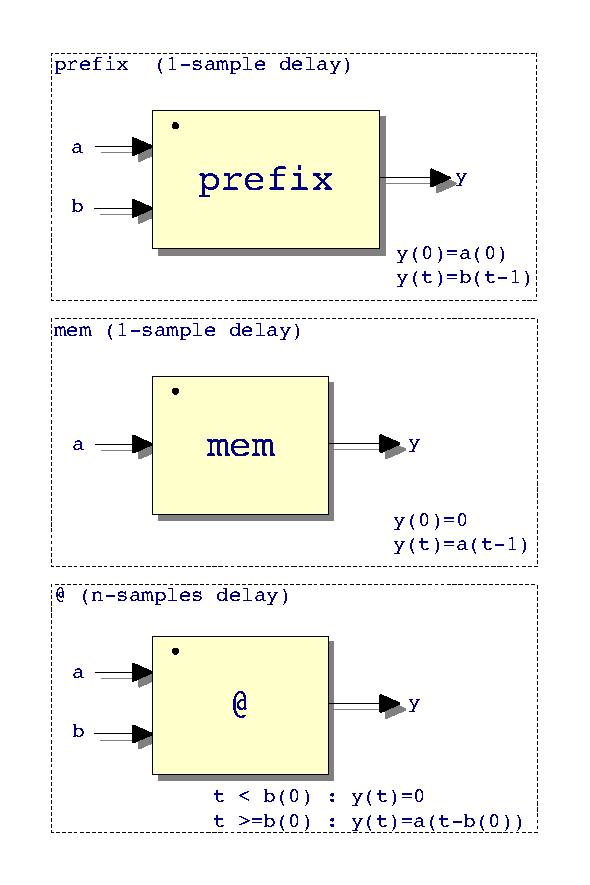
\includegraphics[scale=0.6]{illustrations/faust-diagram4}
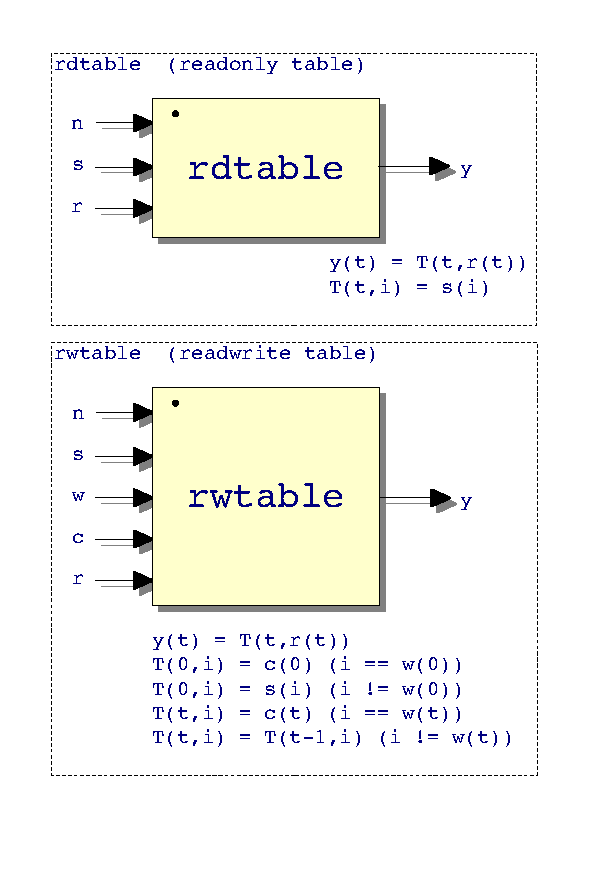
\includegraphics[scale=0.6]{illustrations/faust-diagram5}
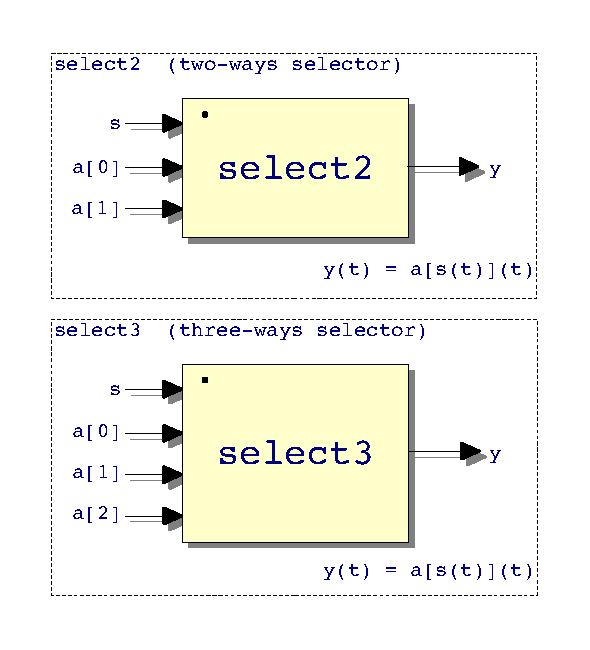
\includegraphics[scale=0.6]{illustrations/faust-diagram6}
\caption{Delays, tables and selectors primitives }
\label{fig:delays}
\end{figure}


%--------------------------------------------------------------------------------------------------------------
\subsection{User Interface Elements}
%--------------------------------------------------------------------------------------------------------------


\faust user interface widgets allow an abstract description of the user interface from within the \faust code. This description is
independent of any GUI toolkits. It is based on \emph{buttons}, \emph{checkboxes}, \emph{sliders}, etc. that are grouped together vertically and
horizontally using appropriate grouping schemes.

All these GUI elements produce signals. A button for example (see figure \ref{fig:button}) produces a signal which is 1 when the button is pressed and 0 otherwise.
These signals can be freely combined with other audio signals.

\begin{figure}[h]
\centering
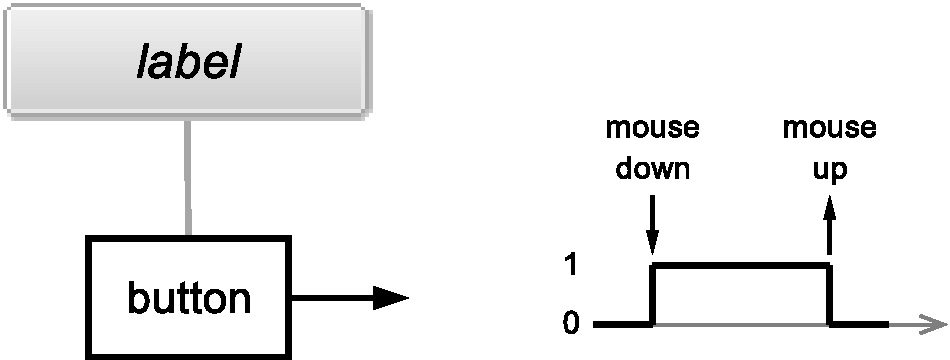
\includegraphics[scale=0.5]{illustrations/button}
\caption{User Interface Button}
\label{fig:button}
\end{figure}


\bigskip

\begin{tabular}{|l|l|}
\hline
\textbf{Syntax} & \textbf{Example} \\
\hline
\texttt{button(\farg{str})} & \texttt{button("play")}\\
\texttt{checkbox(\farg{str})} & \texttt{checkbox("mute")}\\
\texttt{vslider(\farg{str},\farg{cur},\farg{min},\farg{max},\farg{step})} & \texttt{vslider("vol",50,0,100,1)}\\
\texttt{hslider(\farg{str},\farg{cur},\farg{min},\farg{max},\farg{step})} & \texttt{hslider("vol",0.5,0,1,0.01)}\\
\texttt{nentry(\farg{str},\farg{cur},\farg{min},\farg{max},\farg{step})} & \texttt{nentry("freq",440,0,8000,1)}\\
\texttt{vgroup(\farg{str},\farg{block-diagram})} & \texttt{vgroup("reverb", \ldots)}\\
\texttt{hgroup(\farg{str},\farg{block-diagram})} & \texttt{hgroup("mixer", \ldots)}\\
\texttt{tgroup(\farg{str},\farg{block-diagram})} & \texttt{vgroup("parametric", \ldots)}\\
\texttt{vbargraph(\farg{str},\farg{min},\farg{max})} & \texttt{vbargraph("input",0,100)}\\
\texttt{hbargraph(\farg{str},\farg{min},\farg{max})} & \texttt{hbargraph("signal",0,1.0)}\\
\hline
\end{tabular}

\bigskip
\subsubsection{Labels}
Every user interface widget has a label (a string) that identifies it and informs the user of its purpose. There are three important mechanisms associated with labels : \textit{variable parts}, \textit{pathnames} and \textit{metadata}.

\paragraph{Variable parts.}
Labels can contain variable parts. These variable parts are indicated by the sign '\texttt{\%}' followed by the name of a variable. During compilation each label is processed in order to replace the variable parts by the value of the variable. 
For example \lstinline'par(i,8,hslider("Voice %i", 0.9, 0, 1, 0.01))' creates 8 different sliders in parallel :

\begin{lstlisting}
hslider("Voice 0", 0.9, 0, 1, 0.01),
hslider("Voice 1", 0.9, 0, 1, 0.01),
...
hslider("Voice 7", 0.9, 0, 1, 0.01).
\end{lstlisting}

while \lstinline'par(i,8,hslider("Voice", 0.9, 0, 1, 0.01))' would have created only one slider and duplicated its output 8 times.


An escape mechanism is provided.
If the sign \lstinline'%' is followed by itself, it will be included in the resulting string.
For example \lstinline'"feedback (%%)"' will result in \lstinline'"feedback (%)"'.

\paragraph{Pathnames.}
Thanks to horizontal, vertical and tabs groups, user interfaces have a hierarchical structure analog to a hierarchical file system. Each widget has an associated \textit{pathname} obtained by concatenating the labels of all its surrounding groups with its own label.

In the following example :
\begin{lstlisting}
hgroup("Foo",
	...
	vgroup("Faa", 
		...
		hslider("volume",...)
		...
	)
	...
)
\end{lstlisting}
the volume slider has pathname \lstinline'/h:Foo/v:Faa/volume'.

In order to give more flexibility to the design of user interfaces, it is possible to explicitly specify the absolute or relative pathname of a widget directly in its label. 

In our previous example the pathname of :
\begin{lstlisting}
	hslider("../volume",...)
\end{lstlisting}
would have been \lstinline'/h:Foo/volume', while the pathname of :
\begin{lstlisting}
	hslider("t:Fii/volume",...)
\end{lstlisting}
would have been : 
\lstinline'/h:Foo/v:Faa/t:Fii/volume'.

The grammar for labels with pathnames is the following:
\begin{grammar}
  <label> ::= 
  \begin{syntdiag}
	<path> <name>
  \end{syntdiag}
\end{grammar}
%
\begin{grammar}
 <path> ::= 
  \begin{syntdiag}
	\begin{stack} \\ "/" \end{stack} 
	\begin{stack} \\ \begin{rep} <folder> "/" \end{rep} \end{stack} 
 \end{syntdiag}
\end{grammar}
%
\begin{grammar}
 <folder> ::= 
  \begin{syntdiag}
	\begin{stack}
		".." \\ 
		\begin{stack} "h:" \\ "v:" \\ "t:" \end{stack} <name>
	\end{stack}
 \end{syntdiag}
\end{grammar}



\paragraph{Metadata}
Widget labels can contain metadata enclosed in square brackets. These metadata associate a key with a value and are used to provide additional information to the architecture file.  They are tipically used to improve the look and feel of the user interface. 
The \faust code :
\begin{lstlisting}
process = *(hslider("foo [key1: val 1][key2: val 2]", 
					0, 0, 1, 0.1));
\end{lstlisting}

will produce and the corresponding C++ code :

\begin{lstlisting}
class mydsp : public dsp {
	...
	virtual void buildUserInterface(UI* interface) {
	    interface->openVerticalBox("m");
	    interface->declare(&fslider0, "key1", "val 1");
	    interface->declare(&fslider0, "key2", "val 2");
	    interface->addHorizontalSlider("foo", &fslider0, 
								0.0f, 0.0f, 1.0f, 0.1f);
	    interface->closeBox();
	}
...
};
\end{lstlisting}

All the metadata are removed from the label by the compiler and 
transformed in calls to the \lstinline'UI::declare()' method. All these 
\lstinline'UI::declare()' calls will always take place before the \lstinline'UI::AddSomething()' 
call that creates the User Interface element. This allows the 
\lstinline'UI::AddSomething()'  method to make full use of the available metadata.

It is the role of the architecture file to decide what to do with these 
metadata. The \lstinline'jack-qt.cpp' architecture file for example implements the 
following :
\begin{enumerate}
\item \lstinline'"...[type:knob]..."' creates a rotative knob instead of a regular 
slider or nentry.
\item \lstinline'"...[type:led]..."' in a bargraph's label creates a small LED instead 
of a full bargraph
\item \lstinline'"...[unit:dB]..."' in a bargraph's label creates a more realistic 
bargraph with colors ranging from green to red depending of the level of 
the value
\item \lstinline'"...[unit:xx]..."' in a widget postfix the value displayed with xx
\item \lstinline'"...[tooltip:bla bla]..."' add a tooltip to the widget
\end{enumerate}

Moreover starting a label with a number option like in \lstinline'"[1]..."' provide 
a convenient mean to control the alphabetical order of the widgets






%%%%%%%%%%%%%%%%%%%%%%%%%%%%%%%%%%%%%%%%%%%%%%%%%%%%%%%%%%%%%%%%%%%%%%%%%%%%%%%%%%%%%%
%                            INVOKING THE COMPILER                                             %
%%%%%%%%%%%%%%%%%%%%%%%%%%%%%%%%%%%%%%%%%%%%%%%%%%%%%%%%%%%%%%%%%%%%%%%%%%%%%%%%%%%%%%


\chapter{Invoking the \faust compiler}
The \faust compiler is invoked using the \texttt{faust} command. It translate \faust programs into C++ code.
The generated code can be wrapped into an optional \emph{architecture file} allowing to directly produce a fully operational program.

\begin{syntdiag}
compiler : "faust" (options) (file +)
\end{syntdiag}

For example \lstinline'faust noise.dsp' will compile \lstinline'noise.dsp' and output the corresponding C++ code on the standard output.  The option \lstinline'-o' allows to choose the output file : \lstinline'faust noise.dsp -o noise.cpp'. The option \lstinline'-a' allows to choose the architecture file : \lstinline'faust -a alsa-gtk.cpp noise.dsp'. 

To compile a \faust program into an ALSA application on Linux you can use the following commands: 
\begin{lstlisting}
	faust -a alsa-gtk.cpp noise.dsp -o noise.cpp
	g++ -lpthread -lasound  
		`pkg-config --cflags --libs gtk+-2.0` 
		noise.cpp -o noise
\end{lstlisting} 


Compilation options are listed in the following table :

\bigskip

\small
%%\begin{tabularx}{\textwidth}[t]{|l|l|X|}

\tablefirsthead{
\hline
\textbf{Short} 				& \textbf{Long} 					& \textbf{Description}   \\
\hline
}
\tablehead{
\hline
\textbf{Short} 				& \textbf{Long} 					& \textbf{Description}   \\
\hline
}
\tabletail{
  \hline
  \multicolumn{3}{|r|}{\small\sl continued on next page}\\
  \hline
}
\tablelasttail{
  \hline
}


\begin{supertabular}{|p{1.5cm}|p{4cm}|p{5cm}|}  
\texttt{-h} 				& \texttt{--help} 					& print the help message  \\
\texttt{-v} 				& \texttt{--version} 				& print version information  \\
\texttt{-d} 				& \texttt{--details} 				& print compilation details  \\
\texttt{-ps} 				& \texttt{--postscript} 			& generate block-diagram postscript file  \\
\texttt{-svg} 				& \texttt{--svg} 					& generate block-diagram svg files  \\
\texttt{-blur} 				& \texttt{--shadow-blur} 			& add a blur to boxes shadows  \\
\texttt{-sd} 				& \texttt{--simplify-diagrams} 		& simplify block-diagram before drawing them  \\
\texttt{-f \farg{n}} 		& \texttt{--fold \farg{n}}  		& max complexity of svg diagrams before splitting into several files (default 25 boxes)  \\
\texttt{-mns \farg{n}} 		& \texttt{--max-name-size \farg{n}} & max character size used in svg diagram labels\\
\texttt{-sn}             	& \texttt{--simple-names}			& use simple names (without arguments) for block-diagram (default max size : 40 chars) \\
\texttt{-xml} 				& \texttt{--xml} 					& generate an additional description file in xml format  \\
\texttt{-uim} 				& \texttt{--user-interface-macros} 	& add user interface macro definitions to the C++ code  \\
\texttt{-flist} 			& \texttt{--file-list} 				& list all the source files and libraries implied in a compilation  \\
\hline
\texttt{-lb}	 			& \texttt{--left-balanced} 			& generate left-balanced expressions  \\
\texttt{-mb} 				& \texttt{--mid-balanced} 			& generate mid-balanced expressions (default)  \\
\texttt{-rb} 				& \texttt{--right-balanced}			& generate right-balanced expressions  \\
\texttt{-lt} 				& \texttt{--less-temporaries}		& generate less temporaries in compiling delays  \\
\texttt{-mcd \farg{n}}		& \texttt{--max-copy-delay \farg{n}}& threshold between copy and ring buffer delays (default 16 samples)\\
\hline
\texttt{-vec} 				& \texttt{--vectorize}				& generate easier to vectorize code  \\
\texttt{-vs \farg{n}}		& \texttt{--vec-size \farg{n}}		& size of the vector (default 32 samples) when -vec \\
\texttt{-lv \farg{n}}		& \texttt{--loop-variant \farg{n}}	& loop variant [0:fastest (default), 1:simple] when -vec\\
\texttt{-dfs} 				& \texttt{--deepFirstScheduling}	& schedule vector loops in deep first order when -vec \\
\hline
\texttt{-omp} 				& \texttt{--openMP}					& generate parallel code using openMP (implies -vec)  \\
\texttt{-sch} 				& \texttt{--scheduler}				& generate parallel code using threads directly (implies -vec)  \\
\texttt{-g} 				& \texttt{--groupTasks}				& group sequential tasks together when -omp  \\
\hline
\texttt{-single} 			& \texttt{--single-precision-floats} & use floats for internal computations (default)  \\
\texttt{-double} 			& \texttt{--double-precision-floats} & use doubles for internal computations  \\
\texttt{-quad} 				& \texttt{--quad-precision-floats}	&  use extended for internal computations  \\
\hline
\texttt{-mdoc} 				& \texttt{--mathdoc}				& generates the full mathematical description of a \faust program \\
\texttt{-mdlang \farg{l}}			& \texttt{--mathdoc-lang \farg{l}} 		& choose the language of the mathematical description (\farg{l} = en, fr, ...) \\
\texttt{-stripdoc} 			& \texttt{--strip-mdoc-tags}		& remove documentation tags when printing \faust listings\\
\hline
\texttt{-a \farg{file}} 	&  									& architecture file to use  \\
\texttt{-o \farg{file}} 	&  									& C++ output file\\
%%\end{tabularx} 
\end{supertabular} 
\normalsize

\bigskip

The main available architecture files are :

\bigskip

\begin{tabular}{|l|l|l|}
\hline
\textbf{File name}			& \textbf{Description}   \\
\hline
\texttt{jack-gtk.cpp} 		& Jack GTK standalone application  \\
\texttt{jack-qt.cpp} 		& Jack QT4 standalone application  \\
\texttt{jack-console.cpp} 	& Jack command line application  \\
\texttt{jack-internal.cpp} 	& Jack serve plugin  \\
\texttt{jack-wx.cpp} 		& Jack wxWindows standalone application  \\
\texttt{alsa-gtk.cpp} 		& ALSA GTK standalone application  \\
\texttt{alsa-qt.cpp} 		& ALSA QT4 standalone application  \\
\texttt{oss-gtk.cpp} 		& OSS GTK standalone application  \\
\texttt{oss-wx.cpp} 		& OSS wxWindows standalone application  \\
\texttt{pa-gtk.cpp} 		& PortAudio GTK standalone application  \\
\texttt{pa-qt.cpp} 			& PortAudio QT4 standalone application  \\
\texttt{pa-wx.cpp} 			& PortAudio wxWindows standalone application  \\
\hline
\texttt{max-msp.cpp} 		& Max/MSP external  \\
\texttt{vst.cpp} 			& VST plugin  \\
\texttt{vst2p4.cpp} 		& VST 2.4 plugin  \\
\texttt{vsti-mono.cpp} 		& VSTi mono instrument  \\
\texttt{ladspa.cpp} 		& LADSPA plugin  \\
\texttt{q.cpp} 				& Q language plugin  \\
\texttt{supercollider.cpp} 	& SuperCollider Unit Generator  \\
\texttt{csound.cpp} 		& CSOUND opcode  \\
\texttt{puredata.cpp} 		& PD external  \\
\hline
\texttt{sndfile.cpp} 		& sound file transformation command \\
\texttt{bench.cpp} 			& speed benchmark   \\
\texttt{octave.cpp} 		& Octave plugin   \\
\texttt{plot.cpp} 			& Command line application    \\
\texttt{sndfile.cpp} 		& Command line application    \\
\hline
\end{tabular}

\bigskip

Here is an example of compilation command that generates the C++ source code of a Jack application using the GTK graphic toolkit:

\texttt{faust -a jack-gtk.cpp -o freeverb.cpp freeverb.dsp}.

\bigskip

\chapter{Controlling the code generation}
Several options of the \faust compiler allow to control how the C++ code generated. By default the computations are done sample by sample in a single loop. But the compiler can also generate \textit{vector} and \textit{parallel} code.


\section{Vector Code generation}
Modern C++ compilers are able to do autovectorization, that is to use SIMD instructions to speedup the code. These instructions can typically operate in parallel on short vectors of 4 simple precision floating point numbers thus leading to a theoretical speedup of $\times4$. 
Autovectorization of C/C++ programs is a difficult task. Current compilers are very sensitive to the way the code is arranged. In particular too complex loops can prevent autovectorization. The goal of the vector code generation is to rearrange the C++ code in a way that facilitates the autovectorization job of the C++ compiler. Instead of generating a single sample computation loop, it splits the computation into several simpler loops that communicates by vectors.

The vector code generation is activated by passing the \lstinline!--vectorize! (or \lstinline!-vec!) option to the \faust compiler. Two additional options are available:  \lstinline!--vec-size <n>! controls the size of the vector (by default 32 samples) and \lstinline!--loop-variant 0/1! gives some additional control on the loops.  

To illustrate the difference between scalar code and vector code, let's take the computation of the RMS (Root Mean Square) value of a signal.  Here is the \faust code that computes the Root Mean Square of a sliding window of 1000 samples:
\label{rms}
\begin{lstlisting}
// Root Mean Square of n consecutive samples
RMS(n) = square : mean(n) : sqrt ;

// Square of a signal
square(x) = x * x ;

// Mean of n consecutive samples of a signal
// (uses fixpoint to avoid the accumulation of
// rounding errors) 
mean(n) = float2fix : integrate(n) : 
          fix2float : /(n); 

// Sliding sum of n consecutive samples
integrate(n,x) = x - x@n : +~_ ;

// Convertion between float and fix point
float2fix(x) = int(x*(1<<20));      
fix2float(x) = float(x)/(1<<20);    

// Root Mean Square of 1000 consecutive samples
process = RMS(1000) ;
\end{lstlisting}

The compute() method generated in scalar mode is the following:

\begin{lstlisting}
virtual void compute (int count, 
                      float** input, 
                      float** output) 
{
  float* input0 = input[0];
  float* output0 = output[0];
  for (int i=0; i<count; i++) {
    float fTemp0 = input0[i];
    int iTemp1 = int(1048576*fTemp0*fTemp0);
    iVec0[IOTA&1023] = iTemp1;
    iRec0[0] = ((iVec0[IOTA&1023] + iRec0[1])
                    - iVec0[(IOTA-1000)&1023]);
    output0[i] = sqrtf(9.536744e-10f * 
                       float(iRec0[0]));
    // post processing
    iRec0[1] = iRec0[0];
    IOTA = IOTA+1;
  }
}
\end{lstlisting}

The \lstinline!-vec! option leads to the following reorganization of the code:
\begin{lstlisting}
virtual void compute (int fullcount, 
                      float** input, 
                      float** output) 
{
  int     iRec0_tmp[32+4];
  int*    iRec0 = &iRec0_tmp[4];
  for (int index=0; index<fullcount; index+=32) 
  {
    int count = min (32, fullcount-index);
    float* input0 = &input[0][index];
    float* output0 = &output[0][index];
    for (int i=0; i<4; i++) 
      iRec0_tmp[i]=iRec0_perm[i];
    // SECTION : 1
    for (int i=0; i<count; i++) {
      iYec0[(iYec0_idx+i)&2047] =
               int(1048576*input0[i]*input0[i]);
    }
    // SECTION : 2
    for (int i=0; i<count; i++) {
      iRec0[i] = ((iYec0[i] + iRec0[i-1]) - 
               iYec0[(iYec0_idx+i-1000)&2047]);
    }
    // SECTION : 3
    for (int i=0; i<count; i++) {
      output0[i] = sqrtf((9.536744e-10f * 
                 float(iRec0[i])));
    }
    // SECTION : 4
    iYec0_idx = (iYec0_idx+count)&2047;
    for (int i=0; i<4; i++)
      iRec0_perm[i]=iRec0_tmp[count+i];
  }
}
\end{lstlisting}

While the second version of the code is more complex, it turns out to be much easier to vectorize efficiently by the C++ compiler. Using Intel icc 11.0, with the exact same compilation options: \texttt{-O3 -xHost -ftz -fno-alias -fp-model fast=2}, the scalar version leads to a throughput performance of 129.144  MB/s, while the vector version achieves 359.548  MB/s, a speedup of x2.8 ! 

\begin{figure}[htb]
  \centering
  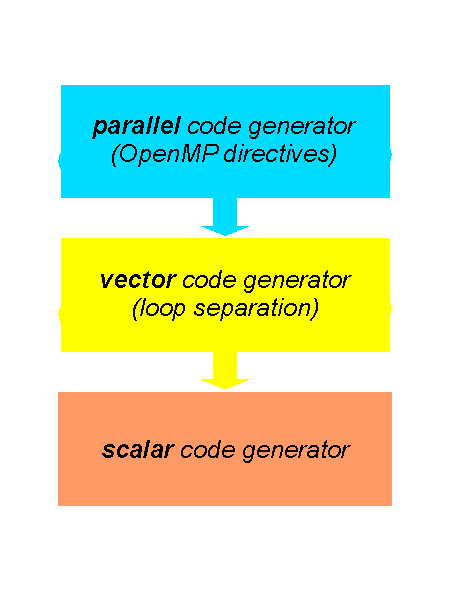
\includegraphics[scale=0.75]{images/compiler-stack}
  \caption{\faust's stack of code generators}   
  \label{fig:stack}
\end{figure}


The vector code generation is built on top of the scalar code generation (see figure \ref{fig:stack}). Every time an expression needs to be compiled, the compiler checks to see if it needs to be in a separate loop or not. It applies some simple rules for that. Expressions that are shared (and are complex enough) are good candidates to be compiled in a separate loop, as well as recursive expressions and expressions used in delay lines. 

The result is a directed graph in which each node is a computation loop (see Figure \ref{fig:loopgraph}). This graph is stored in the klass object and a topological sort is applied to it before printing the code. 

\begin{figure}[htb]
  \centering
  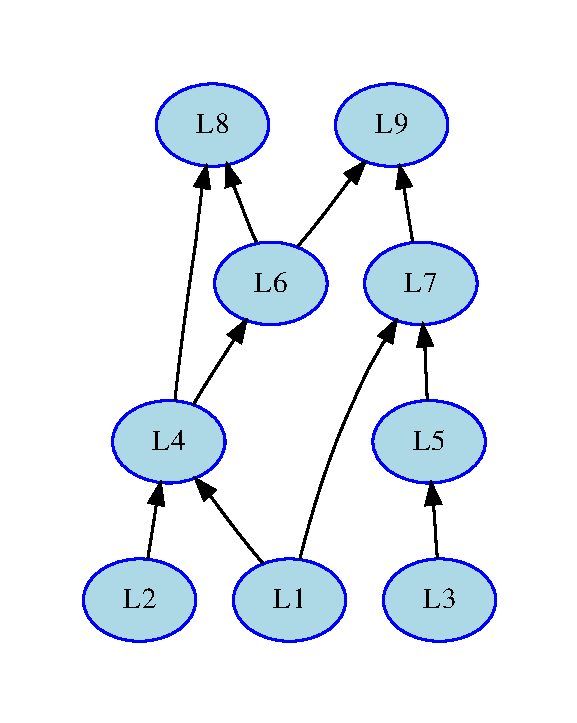
\includegraphics[scale=0.75]{graphs/loopgraph2}
  \caption{The result of the -vec option is a directed acyclic graph (DAG) of small computation loops}   
  \label{fig:loopgraph}
\end{figure}


\section{Parallel Code generation}

The parallel code generation is activated by passing the \lstinline!--openMP! (or \lstinline!-omp!) option to the \faust compiler. It implies the \lstinline!-vec! options as the parallel code generation is built on top of the vector code generation by inserting appropriate OpenMP directives in the C++ code.  

\subsection{The OpenMP API}

\begin{figure}[htb]
  \centering
  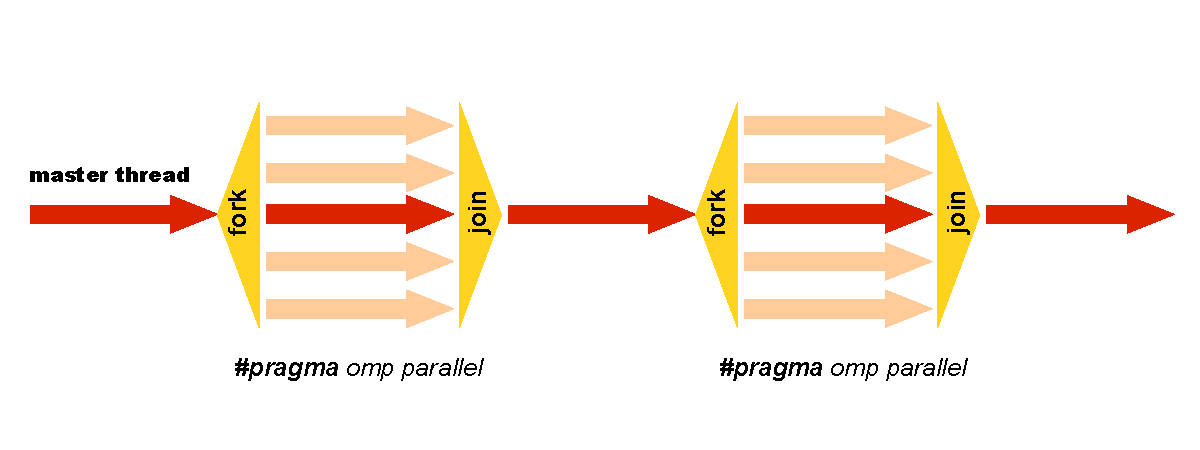
\includegraphics[scale=0.5,angle=-90]{images/openmp-model}
  \caption{OpenMP is based on a fork-join model}   
  \label{fig:openmp}
\end{figure}

OpenMP (http://wwww.openmp.org) is a well established API that is used to explicitly define direct multi-threaded, shared memory parallelism. It is based on a fork-join model of parallelism (see figure \ref{fig:openmp}). 
Parallel regions are delimited by using the \lstinline!#pragma omp parallel! construct. At the entrance of a parallel region a team of parallel threads is activated. The code within a parallel region is executed by each thread of the parallel team until the end of the region. 

\begin{lstlisting}
#pragma omp parallel
{
  // the code here is executed simultaneously by 
  // every thread of the parallel team
  ...
}
\end{lstlisting}

In order not to have every thread doing redundantly the exact same work, OpemMP provides specific \textit{work-sharing} directives. For example \lstinline!#pragma omp sections! allows to break the work into separate, discrete sections. Each section being executed by one thread:

\begin{lstlisting}
#pragma omp parallel
{
  #pragma omp sections
  {
    #pragma omp section
    {
      // job 1
    }
    #pragma omp section
    {
      // job 2
    }
    ...
  }

  ...
}
\end{lstlisting}

\subsection{Adding OpenMP directives}
As said before the parallel code generation is built on top of the vector code generation. The graph of loops produced by the vector code generator is topologically sorted in order to detect the loops that can be computed in parallel. The first set $S_0$ (loops $L1$, $L2$ and $L3$ in the DAG of Figure \ref{fig:loopgraph}) contains the loops that don't depend on any other loops, the set $S_1$ contains the loops that only depend on loops of $S_0$, (that is loops $L4$ and $L5$), etc.. 

As all the loops of a given set $S_n$ can be computed in parallel, the compiler will generate a \lstinline!sections! construct with a \lstinline!section! for each loop. 
\begin{lstlisting}
  #pragma omp sections
  {
    #pragma omp section
    for (...) {
      // Loop 1
    }
    #pragma omp section
    for (...) {
      // Loop 2
    }
    ...
  }
\end{lstlisting}
 
If a given set contains only one loop, then the compiler checks to see if the loop can be parallelized (no recursive dependencies) or not. If it can be parallelized, it generates:
\begin{lstlisting}
  #pragma omp for
  for (...) {
   // Loop code
  }
\end{lstlisting}
otherwise it generates a \lstinline!single! construct so that only one thread will execute the loop:
\begin{lstlisting}
  #pragma omp single
  for (...) {
   // Loop code
  }
\end{lstlisting}

\subsection{Example of parallel code}
To illustrate how \faust uses the OpenMP directives, here is a very simple example, two 1-pole filters in parallel connected to an adder (see figure \ref{fig:parfilter} the corresponding block-diagram):

\begin{lstlisting}
filter(c) = *(1-c) : + ~ *(c);
process = filter(0.9), filter(0.9) : +; 
\end{lstlisting}

\begin{figure}[htb]
  \centering
  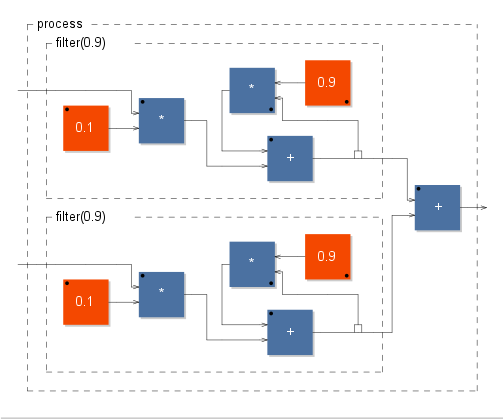
\includegraphics[width=8cm]{images/filter2.png}
  \caption{two filters in parallel connected to an adder}   
  \label{fig:parfilter}
\end{figure}

The corresponding compute() method obtained using the -omp option is the following:
\begin{lstlisting}

virtual void compute (int fullcount, 
                      float** input, 
                      float** output) 
{
  float   fRec0_tmp[32+4];
  float   fRec1_tmp[32+4];
  float*  fRec0 = &fRec0_tmp[4];
  float*  fRec1 = &fRec1_tmp[4];
  #pragma omp parallel firstprivate(fRec0,fRec1)
  {
    for (int index = 0; index < fullcount; 
                                index += 32) 
    {
      int count = min (32, fullcount-index);
      float* input0 = &input[0][index];
      float* input1 = &input[1][index];
      float* output0 = &output[0][index];
      #pragma omp single
      {
        for (int i=0; i<4; i++) 
          fRec0_tmp[i]=fRec0_perm[i];
        for (int i=0; i<4; i++) 
          fRec1_tmp[i]=fRec1_perm[i];
      }
      // SECTION : 1
      #pragma omp sections
      {
        #pragma omp section
        for (int i=0; i<count; i++) {
          fRec0[i] = ((0.1f * input1[i]) 
                   + (0.9f * fRec0[i-1]));
        }
        #pragma omp section
        for (int i=0; i<count; i++) {
          fRec1[i] = ((0.1f * input0[i]) 
                   + (0.9f * fRec1[i-1]));
        }
      }
      // SECTION : 2
      #pragma omp for
      for (int i=0; i<count; i++) {
        output0[i] = (fRec1[i] + fRec0[i]);
      }
      // SECTION : 3
      #pragma omp single
      {
        for (int i=0; i<4; i++) 
          fRec0_perm[i]=fRec0_tmp[count+i];
        for (int i=0; i<4; i++) 
          fRec1_perm[i]=fRec1_tmp[count+i];
      }
    }
  }
}

\end{lstlisting}

This code appeals for some comments:

\begin{enumerate}
\item The parallel construct \lstinline!#pragma omp parallel! is the fundamental construct that starts parallel execution. The number of parallel threads is generally the number of CPU cores but it can be controlled in several ways.

\item Variables external to the parallel region are shared by default. The pragma \lstinline!firstprivate(fRec0,fRec1)! indicates that each thread should have its private copy of fRec0 and fRec1. The reason is that accessing shared variables requires an indirection and is quite inefficient compared to private copies.

\item The top level loop \lstinline!for (int index = 0;...)...! is executed by all threads simultaneously. The subsequent work-sharing directives inside the loop will indicate how the work must be shared between the threads. 

\item Please note that an implied barrier exists at the end of each work-sharing region. All threads must have executed the barrier before any of them can continue.

\item The work-sharing directive \lstinline!#pragma omp single! indicates that this first section will be executed by only one thread (any of them).

\item The work-sharing directive \lstinline!#pragma omp sections! indicates that each corresponding \lstinline!#pragma omp section!, here our two filters, will be executed in parallel.

\item The loop construct \lstinline!#pragma omp for! specifies that the iterations of the associated loop will be executed in parallel. The iterations of the loop are distributed across the parallel threads. For example, if we have two threads, the first one can compute indices between 0 and count/2 and the other between count/2 and count. 

\item Finally \lstinline!#pragma omp single!  in section 3 indicates that this last section will be executed by only one thread (any of them).

\end{enumerate}


\chapter{Mathematical Documentation}

The \faust compiler provides a mechanism to produce a self-describing documentation of the mathematical semantic of a \faust program, essentially as a pdf file. The corresponding options are \lstinline!-mdoc! (short) or \lstinline!--mathdoc! (long).

\section{Goals of the mathdoc}
\label{sec:goals-of-mdoc}

There are three main goals, or uses, of this mathematical documentation:
\begin{enumerate}
\item to preserve signal processors, independently from any computer language but only under a mathematical form;
\item to bring some help for debugging tasks, by showing the formulas as they are really computed after the compilation stage;
\item to give a new teaching support, as a bridge between code and formulas for signal processing.
\end{enumerate}

\section{Generating the mathdoc}
\label{sec:generating-mdoc}

The easiest way to generate the complete mathematical documentation is to call the \lstinline!faust2mathdoc! script on a \faust file (for example: \lstinline!faust2mathdoc noise.dsp!), as the \lstinline!-mdoc! option leave the documentation production unfinished.

\subsection{Invoking the -mdoc option}
\label{sec:invoking-mdoc}

Calling directly \lstinline!faust -mdoc! does only the first part of the work, generating:
\begin{itemize}
\item a top-level directory, suffixed with "\texttt{-mdoc}",
\item 5 subdirectories (\lstinline!cpp/!, \lstinline!pdf/!, \lstinline!src/!, \lstinline!svg/!, \lstinline!tex/!),
\item a \latex file containing the formulas,
\item \textsc{Svg} files for block-diagrams.
\end{itemize}

At this stage:
\begin{itemize}
\item \lstinline!cpp/! remains empty,
\item \lstinline!pdf/! remains empty,
\item \lstinline!src/! contains all \faust sources used (even libraries),
\item \lstinline!svg/! contains \textsc{Svg} block-diagram files,
\item \lstinline!tex/! contains the generated latex file.
\end{itemize}

\subsection{Invoking faust2mathdoc}
\label{sec:invok-faust2m}

The \lstinline!faust2mathdoc! script calls \lstinline!faust --mathdoc! first, then it finishes the work:
\begin{itemize}
\item moving the output C++ file into \lstinline!cpp/!,
\item converting all \textsc{Svg} files into pdf files (you must have a \lstinline!svg2pdf! installed, from the Cairo 2D graphics library),
\item lauching \lstinline!pdflatex! on the \latex file (you must have both \lstinline!pdflatex! and the \lstinline!breqn! package installed),
\item moving the resulting pdf file into \lstinline!pdf/!.
\end{itemize}

\subsection{Examples}
\label{sec:mdoc-examples}

To have an idea of the results of this mathematical documentation, which captures the mathematical semantic of \faust programs, you can look at two pdf files online:
\begin{itemize}
\item \url{http://faust.grame.fr/pdf/karplus.pdf}, for automatic documentation,
\item \url{http://faust.grame.fr/pdf/noise.pdf}, for "manual" documentation.
\end{itemize}

You can also generate all "mdoc" pdfs at once, simply invoking the \lstinline!make mathdoc! command inside the "examples" directory: 
\begin{itemize}
\item a complete "\lstinline!%-mdoc!" directory will be generated for each "\lstinline!%.dsp!" file,
\item a single \lstinline!allmathpdfs! directory will gather all the generated pdf files.
\end{itemize}


\section{Automatic documentation}
\label{sec:auto-docum}

By default, the \lstinline!-mdoc! option generates a \latex file with four sections:
\begin{enumerate}
\item ''Equations of process'', gathering all formulas needed for process,
\item ''Block-diagram schema of process'', showing (only) the top-level block-diagram of process,
\item ''Notice of this documentation'', summing up generation and conventions information,
\item ''Complete listing of the input code'', listing all needed input files (including libraries).
\end{enumerate}


\section{Manual documentation}
\label{sec:manual-mdoc}

You can specify yourself the documentation instead of using the automatic mode, with five xml-like tags. That permits you to modify the presentation and to add your own comments, not only on \lstinline!process!, but also about any sub-process you'd like to. Note that as soon as you declare an \lstinline!<mdoc>! tag inside your \faust file, the default structure of the automatic mode is ignored, and all the \latex stuff becomes up to you!

Here are the five specific tags:
\begin{itemize}
\item \lstinline!<mdoc></mdoc>!, to open a documentation field in your \faust code,
\item \lstinline!<equation></equation>!, to get equations of this specific \faust item,
\item \lstinline!<diagram></diagram>!, to get the top-level block-diagram of this specific \faust item,
\item \lstinline!<notice>!, to insert the "adaptive'' notice all formulas actually printed,
\item \lstinline!<listing>!, to insert the complete listings of all \faust files called.
\end{itemize}


\section{Localization of mathdoc results}
\label{sec:localization-mdoc}

By default, texts used by the documentator are in English, but you can specify another language (French and Italian for the moment), using the \lstinline!-mdlang! option.

If you'd like to contribute to the localization effort, feel free to translate the texts from any of the \lstinline!mathdoctexts-*.txt! files, that are in the \lstinline!architecture! directory (\lstinline!mathdoctexts-fr.txt!, \lstinline!mathdoctexts-it.txt!, etc.).


\chapter{Acknowledgments}
Many persons are contributing to the \faust project by providing code for the compiler, architecture files, libraries, examples, documentation, scripts, bug reports, ideas, etc. I would like in particular to thank :

\begin{itemize}
\item[-]Tiziano Bole	
\item[-]Thomas Charbonnel
\item[-]Damien Cramet
\item[-]Etienne Gaudrin
\item[-]Albert Graef
\item[-]Stefan Kersten
\item[-]Victor Lazzarini
\item[-]Matthieu Leberre
\item[-]Mathieu Leroi
\item[-]Remy Muller
\item[-]Nicolas Scaringella
\item[-]Julius Smith
\end{itemize}


Many developments of the \faust project are now taking place within the ASTREE project (ANR 2008 CORD 003 02) . I would like to thank my ASTREE's partners :
\begin{itemize}
\item[-]J\'er\^ome Barth\'elemy (IRCAM)
\item[-]Alain Bonardi (IRCAM)
\item[-]Raffaele Ciavarella (IRCAM)
\item[-]Pierre Jouvelot (Ecole des Mines/Paristech)
\item[-]Laurent Pottier (U. Saint-Etienne)
\end{itemize}
as well as my colleagues at Grame, in particular : Dominique Fober, Stephane Letz and Karim Barkati.


I would like also to thank for their financial support :
\begin{itemize}
\item[-]the French Ministry of Culture
\item[-]the Rh\^one-Alpes Region
\item[-]the City of Lyon
\item[-]the French National Research Agency (ANR)
\end{itemize}




%%%%%%%%%%%%%%%%%%%%%%%%%%%%%%%%%%%%%%%%%%%%%%%%%%%%%%%%%%%%%%%%%%%%%%%%%%%%%%%%%%%%%%
%%%%%%%%%%%%%%%%%%%%%%%%%%%%%%%%%%%%%%%%%%%%%%%%%%%%%%%%%%%%%%%%%%%%%%%%%%%%%%%%%%%%%%
%                            		END                                              %
%%%%%%%%%%%%%%%%%%%%%%%%%%%%%%%%%%%%%%%%%%%%%%%%%%%%%%%%%%%%%%%%%%%%%%%%%%%%%%%%%%%%%%
%%%%%%%%%%%%%%%%%%%%%%%%%%%%%%%%%%%%%%%%%%%%%%%%%%%%%%%%%%%%%%%%%%%%%%%%%%%%%%%%%%%%%%


\end{document}
